\documentclass[french]{article}
\usepackage[T1]{fontenc}
\usepackage[utf8]{inputenc}
\usepackage{lmodern}
\usepackage[a4paper]{geometry}
\usepackage{babel}
\usepackage{caption}
\usepackage{subcaption}
\usepackage{graphicx}
\graphicspath{{images/}}
\usepackage{float}

\begin{document}
	\begin{center}
		\textbf{\LARGE{Synthèse du mémoire de fin d'études}}
	\end{center}
	
	\begin{center}
		\textbf{\Large{Qilin ZHANG - M2 STL Alternance}}
	\end{center}

	\begin{flushright}
		\large {Septembre 2019}
	\end{flushright}

	\section{Contexte et Problématique}
	Pendant mon alternance, je me suis intégré dans une équipe qui fait les développements et les maintenances d'un produit s'appelle SAP Financial Consolidation (\textit{FC}), le contenu de mon travail est d'automatiser des tests fonctionnels pour ce produit. SAP FC est une application de consolidation légale et de 	reporting de gestion développé depuis 1999. Il permet aux grandes entreprises de répondre à des exigences de consolidation complexes, de rationaliser la conformité réglementaire, d’unifier le reporting légal et de gestion et d’accélérer le processus de clôture financière global. Ce produit plusieurs versions de client comme client sous Windows, client plugin pour Windows Office Excel, client Legacy Web, nouveau client HTML5 Web existe depuis 2015. 
	\paragraph*{}
	L'équipe continue à développer des nouvelles fonctionnalités et faire les maintenances (fixer les bugs) sur FC, ces travaux sont remontés sur différentes branches de codes. Pour assurer la qualité de produit, l'équipe Test fait les tests régressions sur ces nouvelles fonctionnalités et les tests non-régressions sur les fonctionnalités déjà existes. Ces tests peuvent être manuels ou automatisés, après la comparaison entre test manuel et test automatisé dans le mémoire, on peut savoir que le test automatisé est plus pratique pour les tests non-régressions.
	
	\paragraph*{}
	Pour les tests non-régressions, l'équipe Test a déjà développé un projet pour l'automatiser, ce projet utiliser la langage Java et outil Silk Test. Le projet de Test-Auto utilise les machines virtuelles, Jenkins slave, et Perforce afin de lancer les tests et héberger les bases de données que ce dernier aura besoin pendant le tests.
	
	\paragraph*{}
	Pour les tests non-régressions, il y avait la demande de test sur l'impression des rapports, l'objectif est de vérifier si l'impression d'un ou plusieurs mêmes rapports entre différentes versions du client, donne toujours le même résultat, ce dernier est sauvegarder dans les fichiers pdf. Pour ce test, avant je suis arrivé, l'équipe de test a fait manuellement, qui est très fatigant pour les testeurs, et ça va ralentir la procédure du développement. 
	\begin{figure}[H]
		\centering
		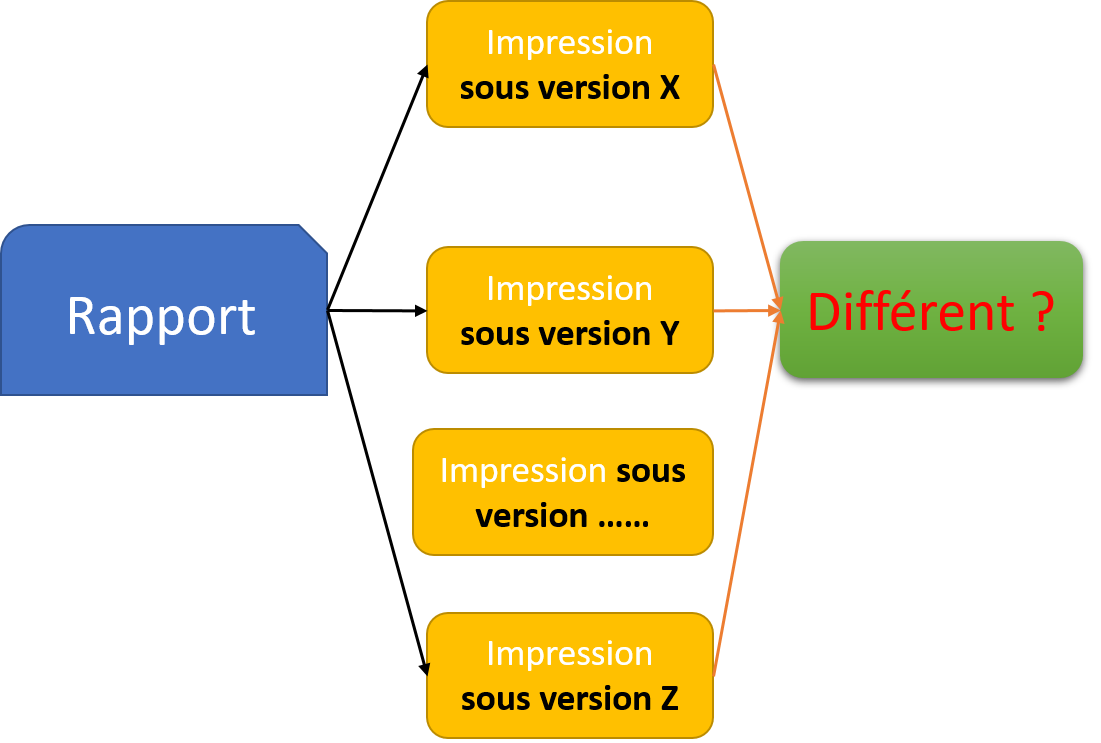
\includegraphics[width=0.43\textwidth]{problematique_print.png}
		\label{fig:prolematique_TestPrint_label}
	\end{figure}
	
	\paragraph*{}
	Avec le contexte et problématique ci-dessus, on m'a demandé d'automatiser les tests d'impressions, ainsi, on m'a demandé aussi d'automatiser d'autres scénarios de tests qui peuvent servir le produit.
	
	\newpage
	\section{Travaux réalisés}	
	\subsection{Comparaison entre deux pdf}
	Pour automatiser les tests d'impressions, l'idée est de réaliser la comparaison entre deux fichiers pdf et visualiser les différences, ensuite les intégrer dans le projet de Test-Auto. 
	
	\paragraph*{}
	Après la communication avec l'autre équipe de SAP France, nous avons trouvé qu'ils ont déjà fait la comparaison entre pdf, mais avec des fonctionnalités plus compliqués, j'ai récupéré leurs codes et adapté dans notre projet en supprimant et simplifié des codes. 
	
	\paragraph*{}
	J'ai lu et compris ce que leurs codes a fait, dans leurs codes, ils transforme d'abord chaque page de pdf en image de format png, puis compare ces images pixel par pixel, ensuite génère les images de format png qui indiquent les différences s'ils sont différents.
	\begin{figure}[H]
		\centering
		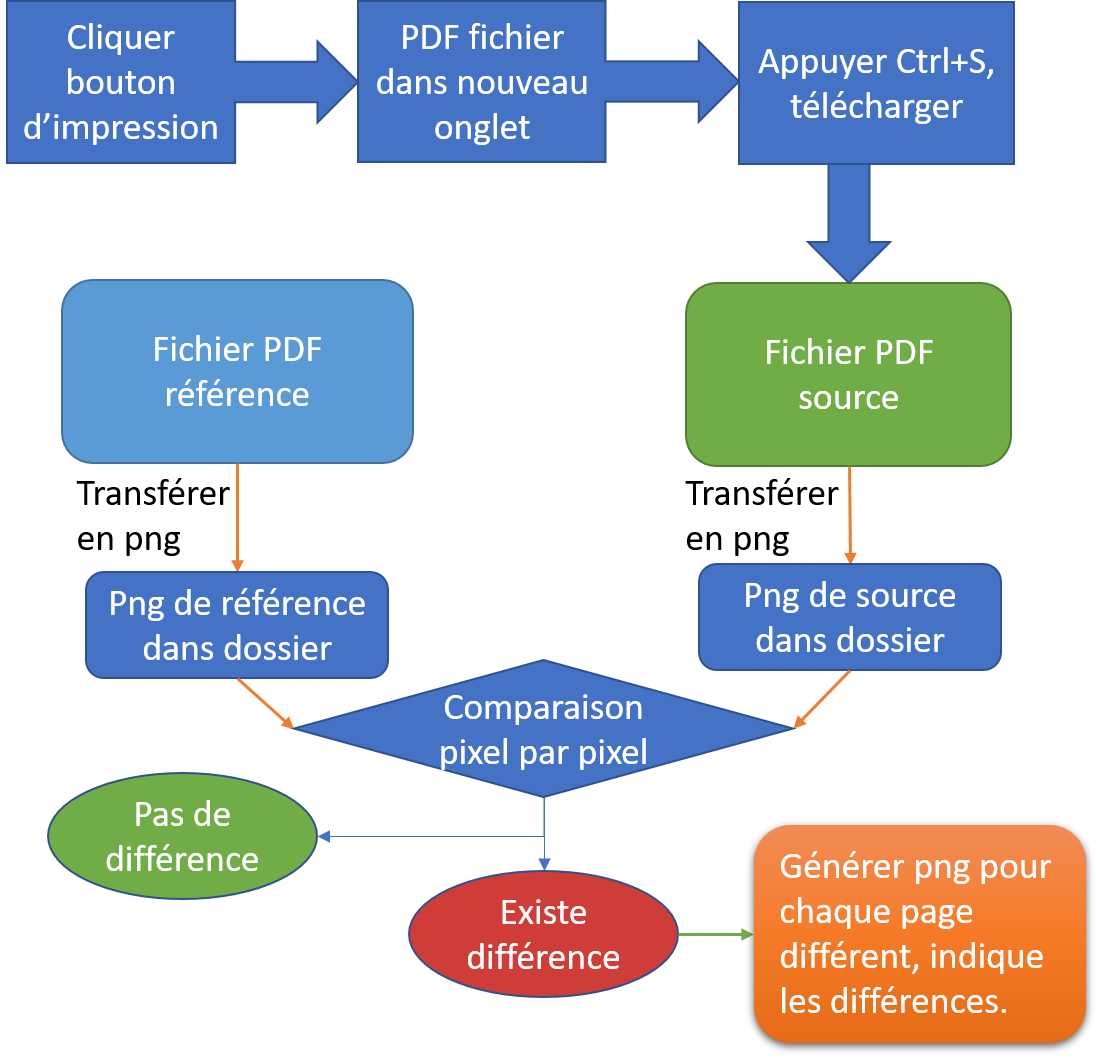
\includegraphics[width=0.48\textwidth]{process_compar_pdf.png}
	\end{figure}
	\subsection{Comparaison les pdfs dans deux dossiers avec lambda expression}
	J'ai été aussi demandé de réaliser la comparaison entre les pdfs dans deux dossiers, je l'ai réalisé avec lambda expression, avec lambda expression, je parcours facilement chaque fichier du premier dossier et fait la comparaison avec les fichiers homonymes qui sont dans le deuxième dossier.
	
	\subsection{Automatiser les tests à l'aide de Xpath}
	SAP Financial Consolidation client HTML5 Web est une application Web, les contrôles d'application  comme bouton, text, checkbox, etc. peuvent être identifiés par \textbf{XPath}. En utilisant Silk Test qui nous permet de reconnaître ces contrôles par \textbf{XPath}, j'ai réalisé également des autres scénarios de tests pendant mon alternance.
	
	\subsection{Les autres nouvelles missions}
	Après la tâche de test d'impression et la soutenance du mémoire, l'équipe va me demander de réaliser d'autres nouvelles tâches, ces tâches resteront toujours sur la partie de Test Automatisé. 
	
\end{document}
